\documentclass{beamer}

\mode<presentation>
{
  \usetheme{% Tema de la presentaci'on (colores, formas, etc.)
    AnnArbor%
    %Antibes%
    %Bergen%
    %Berkeley%
    %Berlin%
    %Boadilla%
    %boxes%
    %CambridgeUS%
    %Copenhagen%
    %Darmstadt%
    %default%
    %Dresden%
    %Frankfurt%
    %Goettingen%
    %Hannover%
    %Ilmenau%
    %JuanLesPins%
    %Luebeck%
    %Madrid%
    %Malmoe%
    %Marburg%
    %Montpellier%
    %PaloAlto%
    %Pittsburgh%
    %Rochester%
    %Singapore%
    %Szeged%
    %Warsaw%
  }

  \setbeamercovered{transparent} % Opcional para la aparicion gradual
}


\usepackage[english]{babel} 

\title{Sistemas de busqueda y ordenamiento}

\subtitle{Shellsort}

\author[Mart\'inez] 
{Gabriel Mart\'{i}nez Gonz\'alez}

\institute[ESFM] 
{
  Escuela Superior de F\'{\i}sica y Matem\'aticas\\
  Instituto Polit\'ecnico Nacional}

\date[\today]{\today}


%\beamerdefaultoverlayspecification{<+->} % Por si se quiere que aparezca
                                          % gradualmente los items


\begin{document}

\begin{frame}
  \titlepage
\end{frame}

\begin{frame}
  \frametitle{Algoritmo de ordenamiento}
  \tableofcontents
\end{frame}

\section{Explicaci\'on del algoritmo}

\begin{frame}
  \frametitle{Ideas principales}
  \framesubtitle{Descripci\'on}
  \begin{itemize}[<+->] % para que parezcan uno a uno
  \item {Es una mejora al algoritmo de inserci\'on directa y burbuja (bubblesort).}
  \item {El algoritmo de inserci\'on o burbuja es muy efectivo con listas casi ordenadas.}
  \item {Se pueden comparar elementos no contiguos.}
  \item {Puede acercar elementos alejados a una posici\'on cercana a la que deber\'{i}a ocupar (ya ordenado).}
  \end{itemize}
\end{frame}

\begin{frame}
  \frametitle{Ideas principales}
  \framesubtitle{Descripci\'on}
  \begin{itemize}[<+->] % para que parezcan uno a uno
  \item {Divide la lista original (de n elementos) en n/2 parejas con un intervalo de n/2 elementos entre ellas y se ordenan.}
  \item {Divide la lista original en n/4 grupos de cuatro elementos con un intervalo de n/4 elementos (y se ordenan).}
  \item {Se repite hasta que se tiene un grupo de n elementos.}
  \item {Dado que ya est\'a "semiordenada" la lista, el m\'etodo de inserci\'on es eficiente.}
  \end{itemize}
\end{frame}

\begin{frame}
  \frametitle{Ideas principales}
  \framesubtitle{Ejemplo}
  \begin{center}
 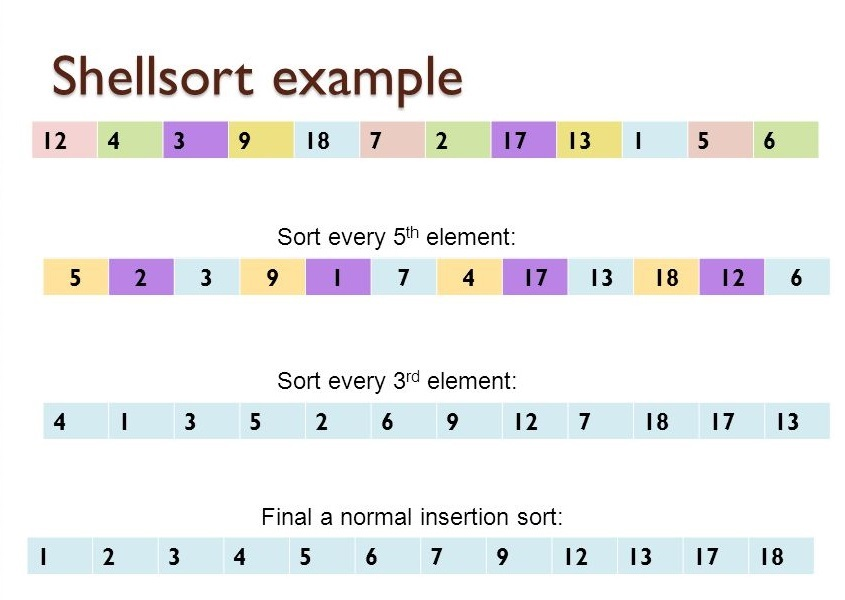
\includegraphics[scale=0.5]{ejemplo}
\end{center}
\end{frame}

\section{Implementaci\'on en c\'odigo}

\begin{frame}
  \frametitle{C\'odigo}
  \framesubtitle{Funci\'on "shell"}
  \begin{center}
 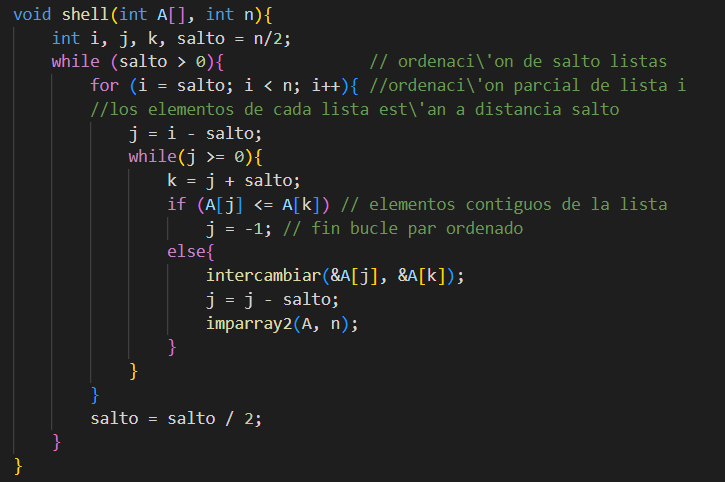
\includegraphics[scale=0.7]{code}
\end{center}
\end{frame}

\section*{Resumen}

\begin{frame}
  \frametitle{Resumen}

  \begin{itemize}
  \item {El ordenamiento Shell es un m\'etodo m\'as eficiente que la inserci\'on.}
  \item {Se organizan elementos separados por varios elementos en el arreglo a ordenar.}
  \end{itemize}
  
\end{frame}


\end{document}

